\documentclass[utf8,dvipsnames,aspectratio=169]{beamer}
\batchmode
% 载入包
\usepackage{amsmath,amssymb,enumerate,epsfig,bbm,calc,color,ifthen,capt-of,multimedia,hyperref}
%\usepackage[orientation=landscape,size=custom,width=16,height=9,scale=0.5]{beamerposter}
\usepackage[UTF8, hyperref]{xeCJK}
\usepackage{fontspec}
\usepackage{color} % documentclass必须加上dvipsnames标签,这一行加没用
\usepackage{indentfirst, ulem}
\usepackage{minted} % 代码高亮,要在XeLaTeX编译里加上-shell-escape -8bit
\usepackage{url} % 链接
\usepackage{relsize}

% 定制主题
\usetheme{Frankfurt}
\useoutertheme[footline=authorinstitute]{miniframes}
% \useoutertheme[subsection=false]{smoothbars}
% \usecolortheme{sustech}

% 设置中文字体
\setCJKmainfont{STKaiti}

% 设置高亮
\newcommand\mk[1]{{\color{RoyalBlue} #1}}

% 贴logo. magic
\pgfdeclareimage[height=3cm]{whu-logo}{figures/whulogo.pdf}
\title{Plotting: HOWTO}
\author{徐来}
\institute{%
	Wuhan University \\
	\pgfuseimage{whu-logo} %
}
\date{\today}

\AtBeginSection[]
{
  \begin{frame}<beamer>
    \frametitle{Outline}
    \tableofcontents[currentsection]
  \end{frame}
}
\beamerdefaultoverlayspecification{<+->}

% -----------------------------------------------------------------------------
\begin{document}
% -----------------------------------------------------------------------------

\frame[plain]{\titlepage}

\begin{frame}{Outline}
  \tableofcontents
\end{frame}

% -----------------------------------------------------------------------------
\section{图表的一般格式要求}
\begin{frame}{图格式}
	\begin{columns}
	\begin{column}<0->{.48\textwidth}
		\begin{figure}[thpb]
			\centering
			\resizebox{.7\linewidth}{!}{
				\includegraphics{figures/fig-1.png}
			}
			\caption{例子}
			\label{fig:ex-fig}
		\end{figure}
	\end{column}
	\begin{column}<0->{.48\textwidth}
		\begin{itemize}
			\item<1-> 灰度或者彩色图
			\item<1-> 四面粗边框
			\item<1-> 刻度有突出
			\item<1-> y轴标题旋转90度
		\end{itemize}
	\end{column}
	\end{columns}
\end{frame}
\begin{frame}{表格式}
	\begin{columns}
	\begin{column}<0->{.48\textwidth}
		\begin{figure}[thpb]
			\centering
			\resizebox{.7\linewidth}{!}{
				\includegraphics{figures/fig-2.png}
			}
			\caption{例子}
			\label{fig:ex-tbl}
		\end{figure}
	\end{column}
	\begin{column}<0->{.48\textwidth}
		\begin{itemize}
			\item<1-> 三线表,边线较粗
			\item<1-> 没有竖线
		\end{itemize}
	\end{column}
	\end{columns}
\end{frame}
\institute{Wuhan University}
\begin{frame}{画图的流程}
	\begin{columns}
    \begin{column}<0->{.24\textwidth}
		\begin{block}<0->{\centering 查看数据的形状}
		\setlength{\parskip}{0.5em}
		\vspace{0.5em}
		首先应该根据实验数据,快速生成草图,这样能够对数据的分布有一个直观的印象
		
		看到数据以后,再来决定用什么图表。
		
		在这一点上\mk{Excel}是非常方便的。
		\vspace{0.5em}
		\end{block}
	\end{column}
	\begin{column}<0->{.24\textwidth}
		\begin{block}{\centering 数据预处理}
		\setlength{\parskip}{0.5em}
		\vspace{0.6em}
		{\color{Red} Raw data -> View}
		
		把结果数据清洗、处理成正式图表的格式。数据太多就需要抽样;太少则要重测或者加值.
		
		\mk{Excel/Ruby}比较方便。\mk{Origin/R}就很僵硬了		
		\vspace{0.6em}		
		\end{block}
	\end{column}
	\begin{column}<0->{.24\textwidth}
		\begin{block}{\centering 画图/调整图表元素}
		\setlength{\parskip}{0.5em}
		\vspace{0.8em}
		画出图表后,要调整\mk{坐标轴、图形、标签和图例}的格式,让它们符合论文要求。
		
		\mk{Origin}的功能强大,更容易画出规范的图表;\mk{R}可以让程序自动生成
		\vspace{0.8em}
		\end{block}	
	\end{column}
	\begin{column}<0->{.24\textwidth}
		\begin{block}{\centering 后期处理}
		\setlength{\parskip}{0.5em}
		\vspace{4em}
		使用\mk{Word/PS/Ai}对图片进行增强和美化
		
		\sout{(还有这种操作!}
		\vspace{4em}
		\end{block}
	\end{column}
	\end{columns}
\end{frame}
% -----------------------------------------------------------------------------
\section{画图工具介绍}
\subsection{Excel}
\begin{frame}{Excel}
	\begin{columns}
	\begin{column}<0->{.48\textwidth}
		\begin{exampleblock}<0->{\centering 优点}
			\vspace{2.4em}
			\begin{itemize}
				\item<0-> 习惯性,画草图方便
				\item<0-> 能够快速看到\mk{数据的形状}
				\item<0-> 方便处理/\mk{筛选}数据,拖放灵活
				\item<0-> 可以集中\mk{暂存}数据,作为其他工具的数据源
				\item<0-> 简单的图可以用Excel完美作出
			\end{itemize}
			\vspace{2.4em}
		\end{exampleblock}
	\end{column}
	\begin{column}<0->{.48\textwidth}
		\begin{alertblock}<0->{\centering 缺点}
			\vspace{1.8em}
			\begin{itemize}
				\item<0-> 图表默认样式不规范需要很多调整,精确度有限
				\item<0-> 无法实现精细的图表格式,例如\mk{科学计数坐标轴,坐标轴截断}等
				\item<0-> 导出基本靠复制粘贴。输出矢量图需要借助\mk{Ai}
				\item<0-> 图复杂了容易崩溃
			\end{itemize}
			\vspace{1.8em}
		\end{alertblock}
	\end{column}
	\end{columns}
\end{frame}
\begin{frame}{Excel图表样例}
	\begin{columns}
	\begin{column}<0->{.48\textwidth}
		\begin{figure}[thpb]
			\centering
			\resizebox{.8\linewidth}{!}{
				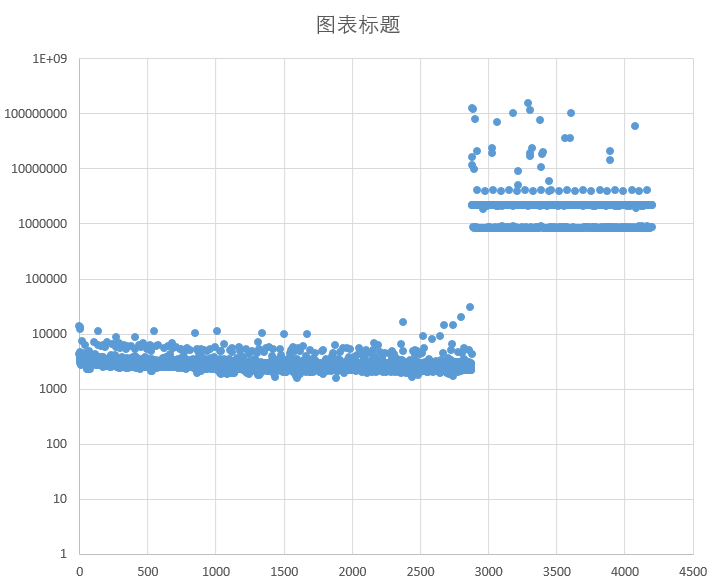
\includegraphics{figures/excel-2.png}
			}
			\caption{自动图表}
			\label{fig:excel-2}
		\end{figure}
	\end{column}
	\begin{column}<0->{.48\textwidth}
		\begin{figure}[thpb]
			\centering
			\resizebox{.9\linewidth}{!}{
				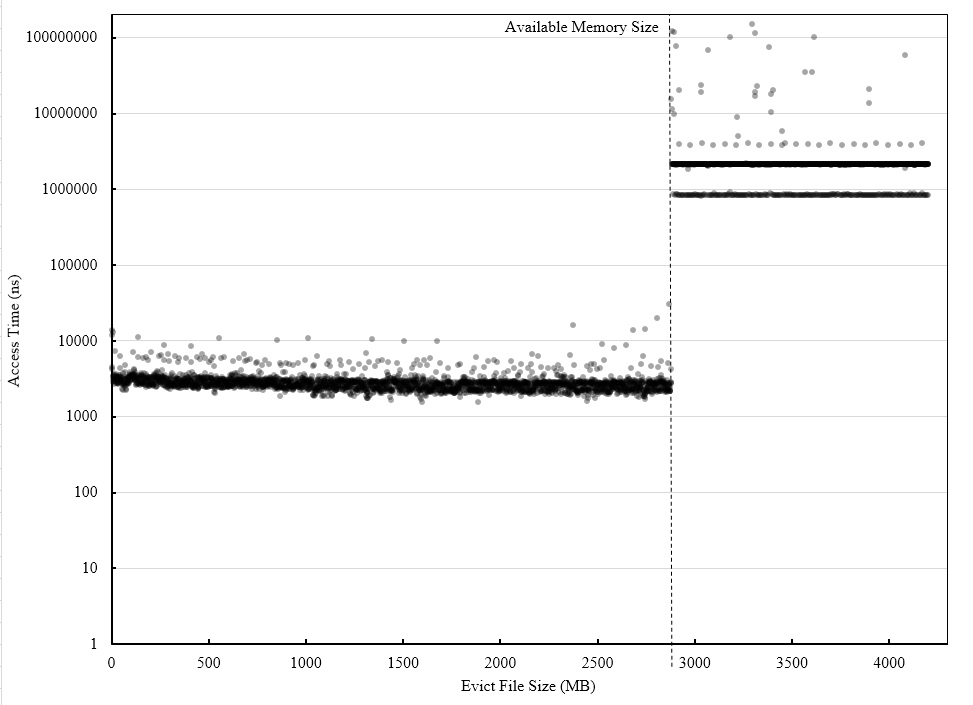
\includegraphics{figures/excel-1.png}
			}
			\caption{修改后}
			\label{fig:excel-1}
		\end{figure}
	\end{column}
	\end{columns}
\end{frame}
\subsection{Matlab/Minitab}
\begin{frame}{Matlab/Minitab}
	\begin{columns}
	\begin{column}<0->{.48\textwidth}
		\begin{exampleblock}<0->{\centering 优点}
			\vspace{2em}
			\begin{itemize}
				\item<0-> 可以直接实现各种算法并且生成图表。函数库丰富
				\item<0-> 图形界面友好,图表处理功能直观
				\item<0-> \mk{Minitab}更轻量,主要用于统计和回归分析
			\end{itemize}
			\vspace{2em}
		\end{exampleblock}
	\end{column}
	\begin{column}<0->{.48\textwidth}
		\begin{alertblock}<0->{\centering 缺点}
			\vspace{2em}
			\begin{itemize}
				\item<0-> 数学、统计函数较多,搞系统一般用不上
				\item<0-> 对matlab环境依赖度大,matlab实现的算法不方便和其他脚本串,慢
				\item<0-> 配色一般般,而且貌似没有抗锯齿
			\end{itemize}
			\vspace{2em}
		\end{alertblock}
	\end{column}
	\end{columns}
\end{frame}
\subsection{Origin}
\begin{frame}{Origin}
	\begin{columns}
	\resizebox{.75\textheight}{!}{
		\begin{column}<0->{.55\textwidth}
			\begin{exampleblock}<0->{\centering 优点}
				\begin{itemize}
					\item<0-> 默认样式规范,可以保存图表模板,将格式快速套用到多个图上(Excel也可)
					\item<0-> 图表元素可供调整的功能非常多,轻松实现\mk{截断/特殊坐标轴/局部缩放}等功能
					\item<0-> 支持抗锯齿(要手动开)和矢量输出
				\end{itemize}
			\end{exampleblock}
			\begin{alertblock}<0->{\centering 缺点}
				\begin{itemize}
					\item<0-> 工作表行列、单元格操作\sout{反人类},最好在Excel里处理好再给他
					\item<0-> 颜色丑,丑,丑
					\item<0-> 偶尔崩溃
				\end{itemize}
			\end{alertblock}
		\end{column}
	}
	\begin{column}<0->{.55\textwidth}
		\begin{figure}[thpb]
			\centering
			\resizebox{.9\linewidth}{!}{
				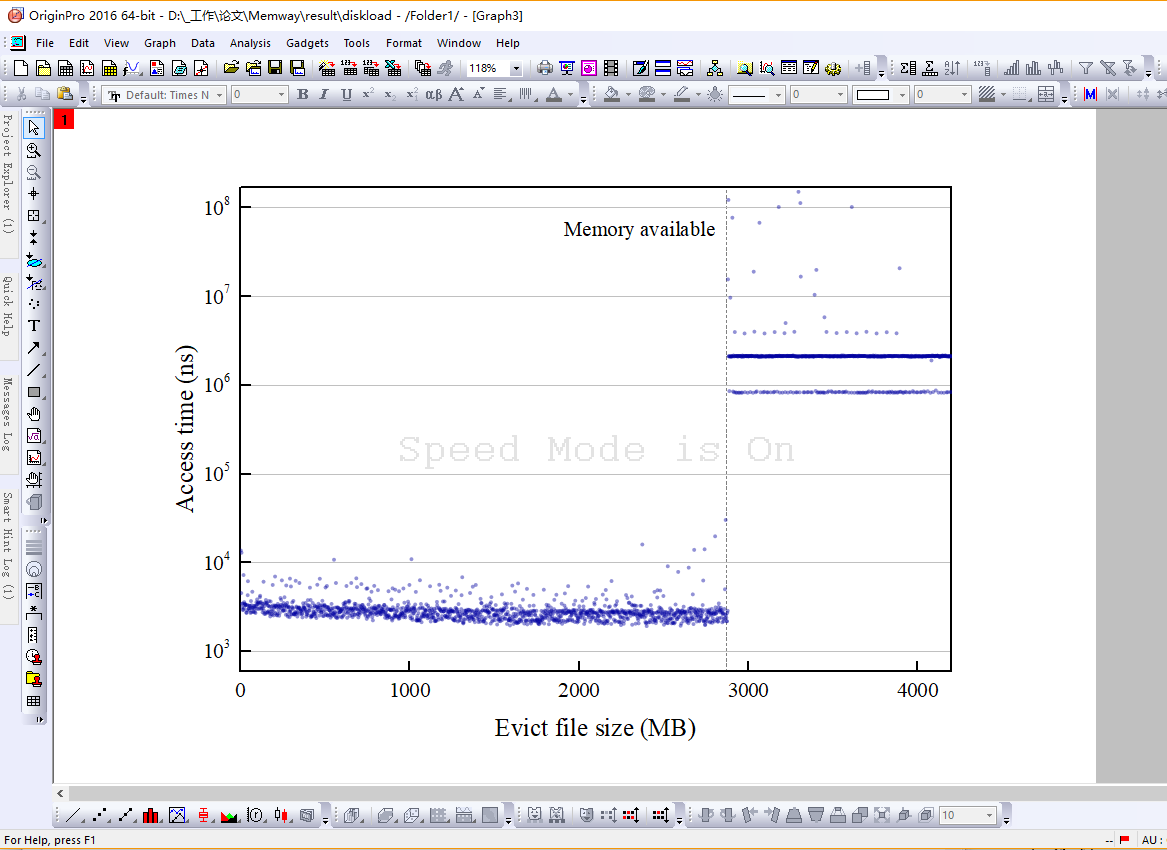
\includegraphics{figures/origin.png}
			}
			\label{fig:origin}
		\end{figure}
	\end{column}
	\end{columns}
\end{frame}
\subsection{R/gnuplot/matplotlib}
\begin{frame}{GNU R / gnuplot / Python matplotlib}
	\begin{columns}
		\begin{column}<0->{.48\textwidth}
			\begin{exampleblock}<0->{\centering 优点}
				\begin{itemize}
					\item<0-> 快速的\mk{数据可视化语言},可以理解为开源免费版Matlab
					\item<0-> 一般使用\mk{ggplot2}库,图表类型丰富,主题配色美观
					\item<0-> 可以在文字中嵌入\mk{Tex公式}
					\item<0-> 方便与其他语言对接,实时处理
					\item<0-> \mk{gnuplot}古老的画图工具,图片像素感较重,一般为系统自带工具使用
					\item<0-> \mk{matplotlib}是python的一个画图库,暂时没用过
				\end{itemize}
			\end{exampleblock}
		\end{column}
		\begin{column}<0->{.48\textwidth}
			\begin{alertblock}<0->{\centering 缺点}
				\vspace{0.5em}
				\begin{itemize}
					\item<0-> R的数据表\mk{(Table/DataFrame)}格式\sout{反人类}
					\item<0-> 大多数csv/json数据载入后要处理成\mk{一维向量}形式才能成图,对数据顺序极为敏感
					\item<0-> 自身有很多统计功能,但是推荐还是在脚本里处理好再给他画图
					\item<0-> ggplot不支持多y轴或者坐标轴截断(作者认为是不规范的画法)
				\end{itemize}
				\vspace{0.5em}
			\end{alertblock}
		\end{column}
	\end{columns}
\end{frame}
\begin{frame}[fragile]{R图表示例} 	% 贴代码时要加fragile选项表明要用外部程序(pygments}处理
	\begin{columns}
		\begin{column}<0->{.56\textwidth}
			\smaller[2]
			\begin{minted}[frame=lines]{R}
result <- fromJSON(file = "access_time_graph_data.json")
fr <- data.frame(result)
m <- melt(fr, id.vars="ticks", 
          variable.name="type", value.name="time")
png("access_time_graph.png", 1280, 640)
    ggplot(m, aes(x=ticks, y=time, fill=type)) +
    geom_bar(stat="identity") +
    theme_economist(base_size=14) + 
    scale_fill_economist()
dev.off()
			\end{minted}
		\end{column}
	\begin{column}<0->{.55\textwidth}
		\begin{figure}[thpb]
			\centering
			\resizebox{.85\linewidth}{!}{
				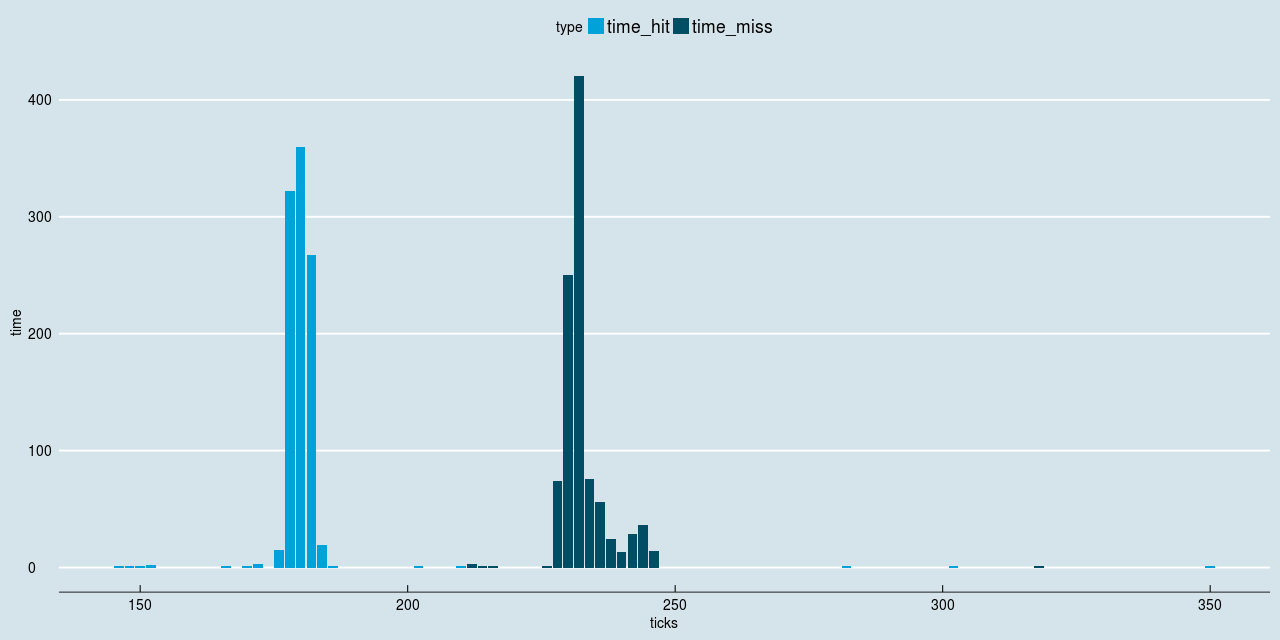
\includegraphics{figures/access_time_graph.png}
			}
			\label{fig:r1}
		\end{figure}
	\end{column}
	\end{columns}
\end{frame}
\begin{frame}[fragile]{R图表示例}
	\begin{columns}
		\begin{column}<0->{.56\textwidth}
			\smaller[2]
			\begin{minted}[frame=lines]{R}
result <- fromJSON(file = "measure_graph_data.json")
data = expand.grid(X=result$X, Y=result$Y)
data$Z = result$Z
png("measure_graph.png", 1024, 1024)
ggplot(data, aes(X, Y, z=Z)) +
    geom_tile(aes(fill=Z)) +
    geom_text(aes(label=Z, alpha=Z)) +
    scale_fill_gradient(low="white", high="blue") +
    theme_economist()
dev.off()
			\end{minted}
		\end{column}
	\begin{column}<0->{.55\textwidth}
		\begin{figure}[thpb]
			\centering
			\resizebox{.75\linewidth}{!}{
				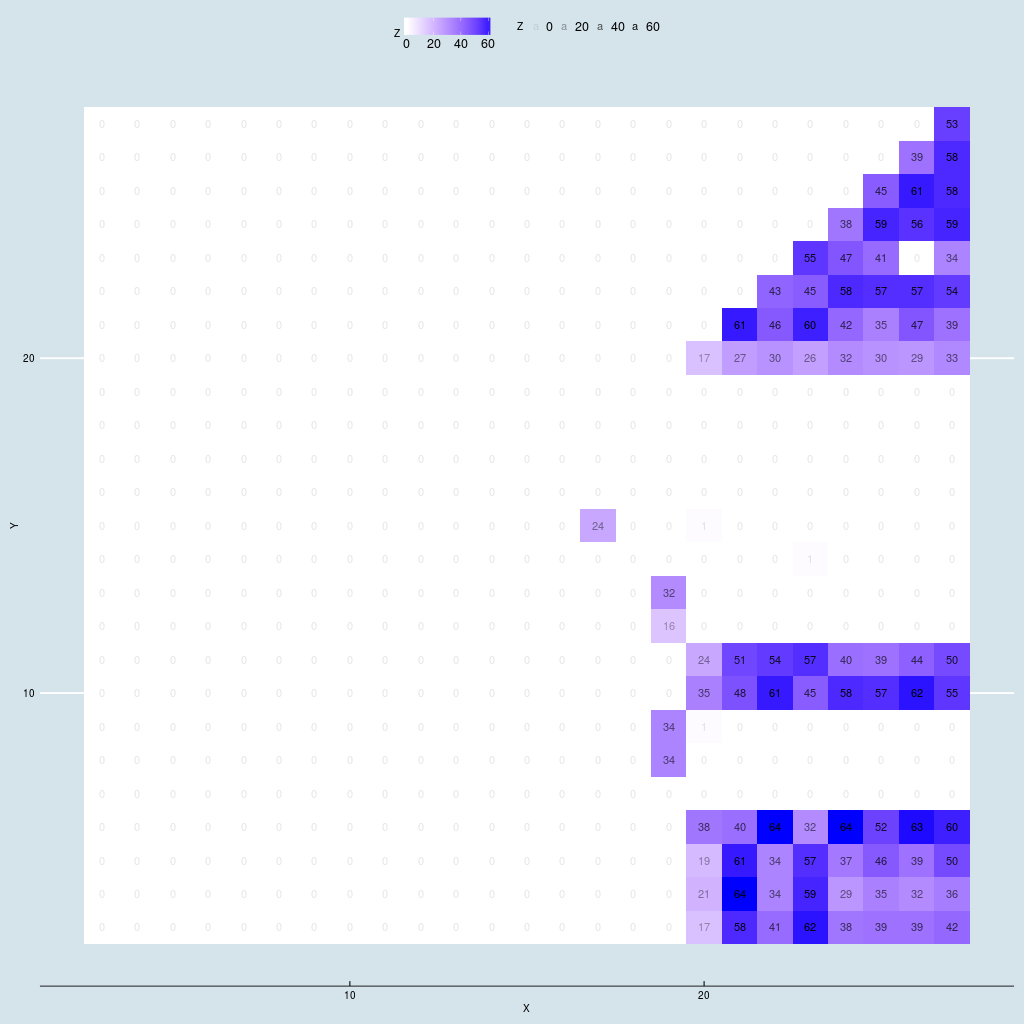
\includegraphics{figures/measure_graph.png}
			}
			\label{fig:r2}
		\end{figure}
	\end{column}
	\end{columns}
\end{frame}
\subsection{Visio}
\begin{frame}{Visio}
	\begin{columns}
		\begin{column}<0->{.48\textwidth}
			\begin{block}<0->{}
				\begin{itemize}
					\item<0-> 除了图表以外,结构图和流程图也是论文中重要的图形内容,一般为灰度图,称为\mk{Line Art}
					\item<0-> \mk{Visio}制作这种图形是相当方便的,就是要对\mk{线型和字形}做较多的调整。
					\item<0-> 注意让图形尽量\mk{紧凑},减少不必要的空白和间隔区域
					\item<0-> \mk{Graphviz}没试过
				\end{itemize}
			\end{block}
		\end{column}
	\begin{column}<0->{.48\textwidth}
		\begin{figure}[thpb]
			\centering
			\resizebox{.9\linewidth}{!}{
				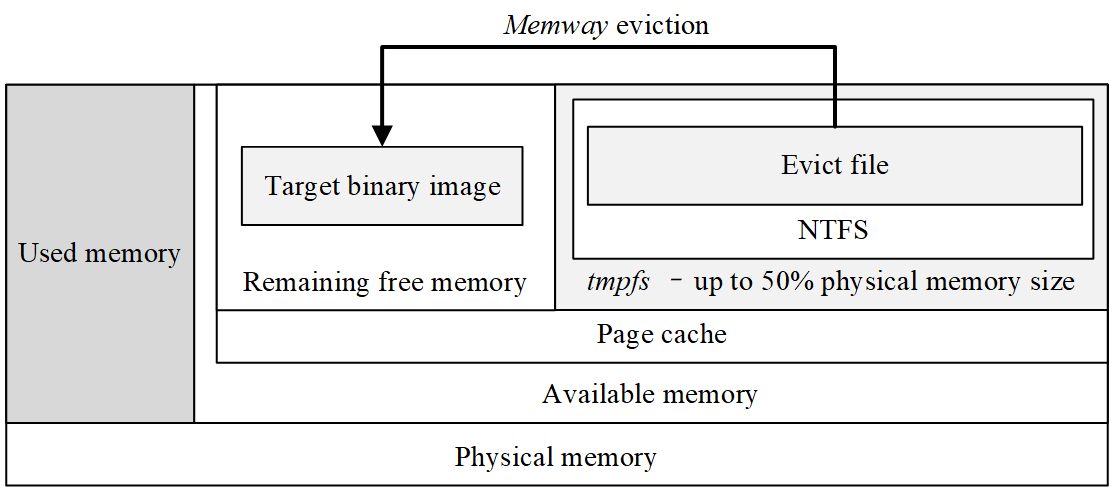
\includegraphics{figures/visio.png}
			}
			\label{fig:visio}
		\end{figure}
	\end{column}
	\end{columns}
\end{frame}
\subsection{Illustrator}
\begin{frame}{Adobe Illustrator}
	\begin{columns}
		\begin{column}<0->{.48\textwidth}
			\begin{block}<0->{}
				\begin{itemize}
					\item<0-> 矢量图的PS,具体应用还需尝试
					\item<0-> 可以对Origin/R之类的软件输出的矢量图进行抗锯齿、后期美化等操作。
					\item<0-> 可以输出成各种图像格式和pdf
				\end{itemize}
			\end{block}
		\end{column}
	\begin{column}<0->{.48\textwidth}
		\begin{figure}[thpb]
			\centering
			\resizebox{.9\linewidth}{!}{
				
\includegraphics{figures/ai.png}
			}
			\label{fig:ai}
		\end{figure}
	\end{column}
	\end{columns}
\end{frame}

\section{\LaTeX-Beamer介绍}
\begin{frame}{关于\LaTeX}
	\begin{block}{1. 怎么跑起来?}
	\small 我用的是直接安装的\mk{Texlive}。很重但是扩展包和编译工具很齐全。Linux下待补充。
	\end{block}
	\begin{block}{2. 如果只是想生成公式呢?}
	\small 可以直接用在线的latex公式编辑器。比如
	\mk{\url{http://www.codecogs.com/latex/eqneditor.php}}
	\begin{figure}[thpb]
	\centering
	\resizebox{.4\linewidth}{!}{
		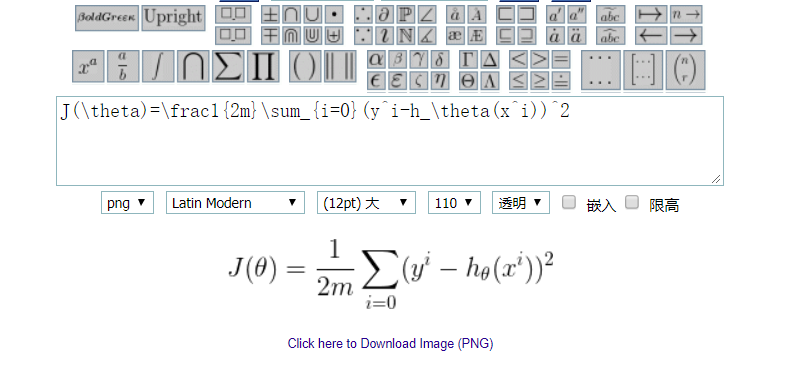
\includegraphics{figures/eq.png}
	}
	\label{fig:ai}
	\end{figure}
	\end{block}
	
\end{frame}
\begin{frame}{关于\LaTeX}
	\smaller[2]
	\begin{block}{3. 怎么做ppt?}
	根据latex的文档类型(documentclass),有不同的核心模板文档类。例如\mk{beamer}就是演示稿,\mk{IEEETran}就是文章,之类的。还有各种\mk{毕业论文}的模板。
	需要注意的是,毕业论文模板和学院的格式要求多少是有出入的,不过一般也在容忍范围内。
	\end{block}
	\begin{block}{4. 大概的流程}
		\begin{itemize}
			\item<0-> \mk{git clone}初始模板,编译一下(排版),弄一个\mk{清理中间文件}的Makefile或者脚本
			\item<0-> 对主题进行一些微调,让他更符合自己的习惯
			\item<0-> 使用XE\LaTeX 编译,虽然比较慢但是对\mk{中文和字体}支持较好。默认的pdflatex过于古老,不合适
			\item<0-> \mk{多多尝试}
		\end{itemize}
	\end{block}	
	\begin{alertblock}{5. 需要注意的}
		使用\LaTeX 制作文档和ppt虽然讲究,但是要多花很多的时间和精力去踩坑。所以并不适合快速展示。
		
		更适合的场合是类似会议、正式报告等需要产品级品质的学术展示时。\mk{平时怎么快怎么来。}
	\end{alertblock}	
\end{frame}

\begin{frame}[plain]{Q\&A}
  \begin{center}
    \Huge Q\&A
  \end{center}
\end{frame}

% -----------------------------------------------------------------------------
\end{document}
